% ====================================================================
\chapter{Pruebas, Resultados y Discusión}
\label{cap:pruebas_resultados_discusion}
% ====================================================================

\section{Corpus y metodología de adquisición de datos de LSA}
% todo: Para mi, habria que decir que lo de ASL solo fue para probar arquitecturas de clasificacion, pero se sabia que no era el dataset final, puesto que nuestro objetivo es un corpus LSA.
El desarrollo del módulo de reconocimiento comenzó con un conjunto de prueba de la Lengua de Señas Americana (ASL). Ese material sirvió para poner a punto el pipeline inicial de extracción y de clasificación, antes de contar con grabaciones propias. La línea se descartó en las primeras iteraciones por dos motivos. El primero es lingüístico: la ASL no es intercambiable con la LSA, porque difiere en el léxico, en la gramática y, en varios ítems, en la forma de la seña. El segundo es de calidad: el conjunto presentaba etiquetas inconsistentes y videos espejados. El antecedente local LSA64, por su parte, emplea un protocolo de captura controlada con guantes de colores, una condición que no se reproduce en una videollamada con cámara web doméstica. Por esas razones, el entrenamiento usa un corpus propio de Lengua de Señas Argentina (LSA).

\subsection{Definición y validación del vocabulario de 100 clases}
% TODO: Ponemos a miriam o a ASNAR?
El vocabulario objetivo abarca un conjunto de 100 señas delimitadas con el asesoramiento técnico de un informante calificado en LSA. La selección léxica priorizó dos dominios funcionales: identificación de personas y verbos de emergencia, por un lado, y asistencia al viajero (indicadores temporales, lugares, parentesco y saludos), por el otro.

La incorporación de las clases al modelo operó de manera condicionada al alcance de un piso mínimo de muestras en el dataset. En julio de 2026, con un umbral de 50 videos por clase, el modelo activo clasificó 91 señas. En agosto de 2026, el incremento del piso a 60 videos permitió incorporar las señas \texttt{chau}, \texttt{tener} y \texttt{años}. El conjunto llegó así a 94 clases. En septiembre de 2026, el conjunto se consolidó en 97 clases mediante la adición de \texttt{pasado}, \texttt{futuro} y \texttt{mio}. En octubre de 2026 el vocabulario se cerró en 100 clases con \texttt{gracias}, \texttt{ayudar} y \texttt{policia}, y completando todas las señas con 100 muestras.

Las 100 glosas se categorizan en: partículas interrogativas, afirmación y negación, dígitos, alfabeto dactilológico, pronombres, saludos, unidades temporales, relaciones de parentesco, lugares y un conjunto cerrado de verbos.

\subsection{Protocolo de grabación y curación del dataset propio}
La captura de video se ejecutó en resolución $1920 \times 1080$ píxeles con relación de aspecto 16:9. A fecha de septiembre de 2026, el dataset contabilizó 6\,748 archivos en formato MP4 (promedio de 69 clips por seña) y 6\,680 tensores en formato \texttt{.npy} con dimensiones $(16, 225)$ guardados en el directorio \texttt{dataset\_landmarks\_16frames}. 

Para evitar desbalances, la selección de muestras limitó el cupo a un máximo de 60 clips por clase mediante aleatorización con semilla fija (42). La partición de datos reservó el 80\,\% de las secuencias para entrenamiento y el 20\,\% para validación, es decir, 48 y 12 clips por clase respectivamente. En el checkpoint del 15 de septiembre de 2026, este esquema totalizó 4\,656 secuencias de entrenamiento y 1\,164 de validación. Con el vocabulario de 100 clases, el mismo esquema produjo 4\,800 secuencias de entrenamiento y 1\,200 de validación (reentrenamiento del 15 de octubre de 2026).

Dado que la partición operó por clip y no por sujeto, secuencias registradas en una misma sesión de grabación se distribuyeron entre ambos conjuntos. Este factor explica por qué la exactitud observada en la fase de validación fuera de línea resultó superior a las mediciones obtenidas posteriormente frente a la cámara en tiempo real.

La aumentación de datos se aplicó exclusivamente durante la fase de entrenamiento mediante transformaciones al vuelo:
\begin{itemize}
    \item Escala isotrópica aleatoria en el rango de $0{,}85$ a $1{,}15$.
    \item Ruido gaussiano sobre las coordenadas, con desvío de $0{,}012$ en los puntos de pose y de $0{,}027$ en los de las manos.
    \item Rotación tridimensional (ángulos de guiñada o \textit{yaw} $\pm 15^{\circ}$, cabeceo o \textit{pitch} y balanceo o \textit{roll} $\pm 8^{\circ}$).
    \item Recorte temporal aleatorio de hasta un 15\,\% en los extremos de la secuencia.
    \item Deformación de velocidad de articulación en el rango de $0{,}80$ a $1{,}25$.
    \item Anulación aleatoria de hasta 3 fotogramas consecutivos con posterior interpolación lineal.
\end{itemize}

Un multiplicador virtual de factor 25 generó variaciones estocásticas en cada época de entrenamiento. Se omitió la inversión horizontal (\textit{flipping}) para preservar la lateralidad nativa de las señas asimétricas. El conjunto de validación no recibió aumentaciones ni repeticiones sintéticas.

\section{Evaluación empírica del clasificador gestual (TinySkeletonClassifier)}

El criterio de selección del modelo integrado en el producto final no respondió a la exactitud de validación fuera de línea, sino al porcentaje de aciertos en la evaluación frente a la cámara local en vivo (modos Top-1 y Top-3, una toma por seña, mano diestra y modo automático). A lo largo del desarrollo, esta métrica orientó el descarte de redes de mayor complejidad, búsquedas automatizadas de hiperparámetros y líneas de aprendizaje por transferencia, y ratificó la elección del modelo base de 16 fotogramas.

\subsection{Protocolo de evaluación en cámara real}
\label{sec:protocolo_camara}
La prueba de integración se ejecutó en la estación local mediante un script interactivo que solicitó la articulación consecutiva de las señas del vocabulario. El clasificador emitió la glosa predicha junto con su nivel de confianza. Esta evaluación enfrentó al modelo a variaciones de iluminación, óptica y posicionamiento no presentes en el conjunto de entrenamiento.

\subsection{Comparativa entre métricas fuera de línea y rendimiento en cámara}
La Tabla~\ref{tab:brecha_offline_camara} presenta la brecha sistemática entre la exactitud obtenida en validación estática y el rendimiento registrado en tiempo real.

\begin{table}[H]
    \centering
    \small
    \caption{Exactitud de validación fuera de línea frente al acierto en cámara real (Top-1 y Top-3 crudos, sin colapsar homógrafos).}
    \label{tab:brecha_offline_camara}
    \begin{tabular}{llccc}
        \toprule
        \textbf{Checkpoint} & \textbf{Fecha} & \textbf{Val. Top-1} & \textbf{Cámara Top-1} & \textbf{Cámara Top-3} \\
        \midrule
        16 fotogramas, 91 clases & 29--30/07 & 97{,}36\,\% & 61{,}5\,\% & 83{,}5\,\% \\
        32 fotogramas, 128/4/2 & 31/07 & 96{,}48\,\% & 71{,}4\,\% & 87{,}9\,\% \\
        32 fotogramas, 64/2/1 & 31/07 & 97{,}36\,\% & 67{,}0\,\% & 90{,}1\,\% \\
        Optuna v1, 32 fotogramas & 31/07 & 97{,}69\,\% & 66{,}0\,\% & 84{,}6\,\% \\
        Baseline 16f, luz ambiental, 94 clases & 18/08 & 98{,}40\,\% & 67{,}0\,\% & 89{,}4\,\% \\
        Baseline 16f, iluminación dirigida, 94 clases & 28/08 & 98{,}40\,\% & 86{,}2\,\% & 95{,}7\,\% \\
        Baseline 16f, 97 clases & 15--17/09 & 98{,}28\,\% & 77{,}3\,\% & 94{,}8\,\% \\
        \bottomrule
    \end{tabular}
\end{table}

Tres factores explican esta diferencia:
\begin{enumerate}
    \item \textbf{Disparidad de dominio:} La validación reutilizó encuadres de los videos originales, mientras que la cámara web del cliente introdujo ópticas y distorsiones distintas.
    \item \textbf{Sensibilidad a la iluminación:} La misma arquitectura de 16 fotogramas incrementó su rendimiento en cámara del 67{,}0\,\% al 86{,}2\,\% Top-1 al controlar la iluminación del entorno (sesión del 28 de agosto), sin modificar los pesos de la red.
    \item \textbf{Varianza por toma única:} Evaluaciones repetidas sobre un conjunto de 36 caracteres evidenciaron fluctuaciones de entre 11 y 19 puntos porcentuales asociadas a la variabilidad de articulación en una sola toma.
\end{enumerate}

En paralelo, se evaluó una línea de aprendizaje por transferencia (\textit{Transfer Learning}) sobre coordenadas articulares que alcanzó exactitudes de 0,98 y 0,99 en reportes estáticos sobre 1\,084 muestras. No obstante, esos reportes incluían clases sin soporte y no completaron el protocolo de evaluación en cámara, por lo que la aproximación se descartó a favor del modelo \textit{TinySkeleton} entrenado desde cero.

\subsection{Impacto de la resolución temporal: 16 frente a 32 fotogramas}
En julio de 2026, con un vocabulario de 91 clases y 50 videos por clase, se evaluó la hipótesis de que un mayor contexto temporal (32 fotogramas) mejoraría la discriminación de gestos dinámicos extensos. En la Tabla~\ref{tab:frames_julio} y las Figuras~\ref{fig:curva_16} y~\ref{fig:curva_32} se detallan los resultados obtenidos.

\begin{table}[H]
    \centering
    \small
    \caption{Evaluación de la resolución temporal en julio de 2026 (91 clases, 50 videos por clase).}
    \label{tab:frames_julio}
    \begin{tabular}{lcccc}
        \toprule
        \textbf{Iteración} & \textbf{Arquitectura} & \textbf{Val. Top-1} & \textbf{Cámara Top-1} & \textbf{Cámara Top-3} \\
        \midrule
        A, 16 fotogramas & 128 dim / 4 cabezas / 2 capas & 97{,}36\,\% & 61{,}5\,\% & 83{,}5\,\% \\
        B, 32 fotogramas & 128 dim / 4 cabezas / 2 capas & 96{,}48\,\% & 71{,}4\,\% & 87{,}9\,\% \\
        C, 32 fotogramas & 64 dim / 2 cabezas / 1 capa & 97{,}36\,\% & 67{,}0\,\% & 90{,}1\,\% \\
        \bottomrule
    \end{tabular}
\end{table}

\begin{figure}[H]
    \centering
    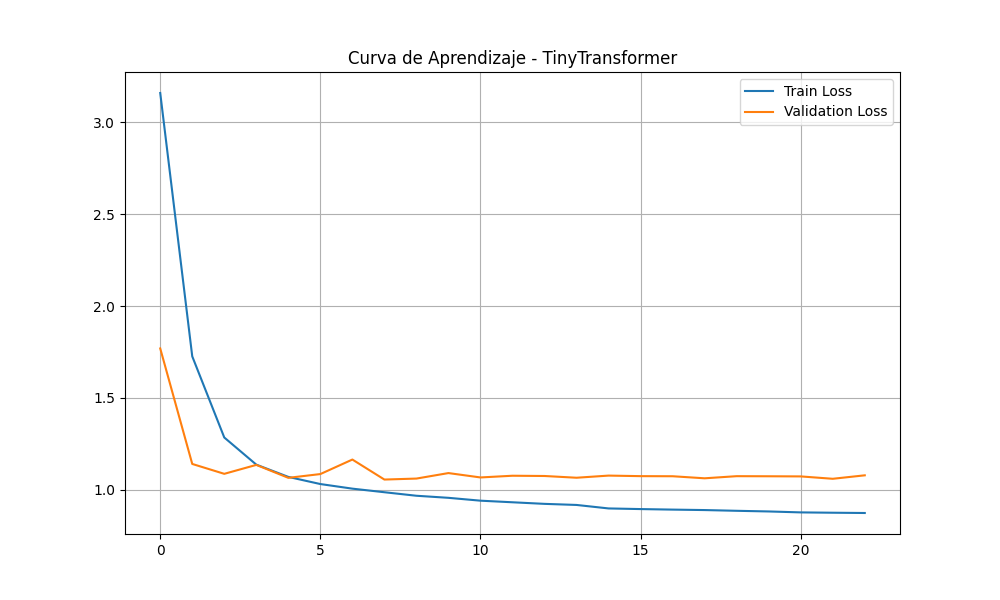
\includegraphics[width=0.82\textwidth]{clasificador/curva_16_frames.png}
    \caption{Curva de aprendizaje para la iteración A (16 fotogramas, 29/07/2026). La pérdida de validación se estabiliza cerca de $1{,}05$ desde la época 7, mientras la pérdida de entrenamiento sigue en descenso.}
    \label{fig:curva_16}
\end{figure}

\begin{figure}[H]
    \centering
    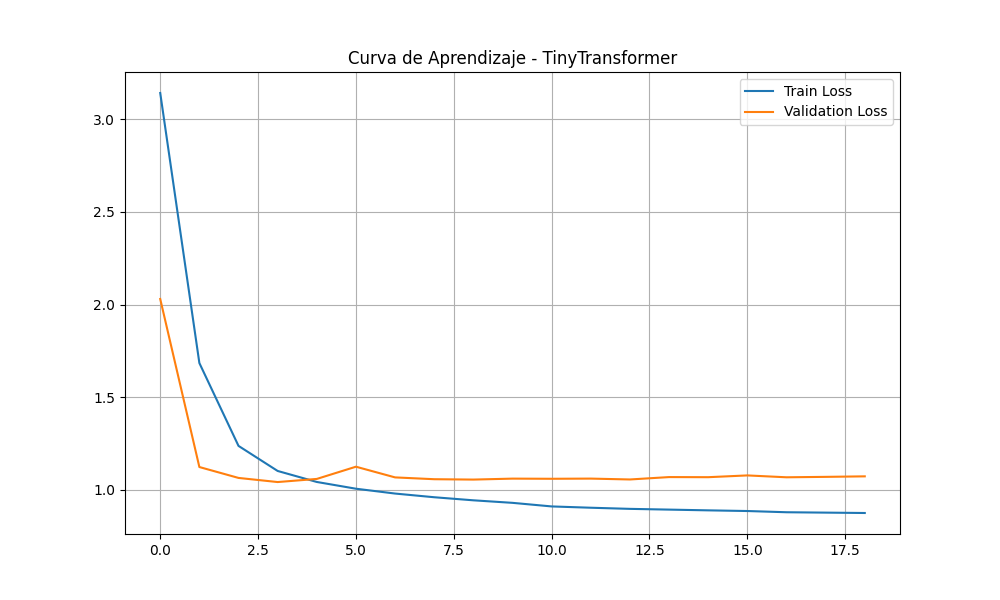
\includegraphics[width=0.82\textwidth]{clasificador/curva_32_frames_b.png}
    \caption{Curva de aprendizaje para la iteración B (32 fotogramas, 128 dimensiones, 4 cabezas y 2 capas, 31/07/2026). La pérdida de validación alcanza la estabilidad en $1{,}04$ desde la época 4.}
    \label{fig:curva_32}
\end{figure}

En las pruebas iniciales de julio, la ventana de 32 fotogramas aportó una ganancia de 9,9 puntos en el Top-1 frente a la cámara (71{,}4\,\% frente a 61{,}5\,\%). Sin embargo, a partir de agosto, con la expansión del dataset a 60 muestras por clase y la incorporación de aumentaciones avanzadas, la comparación favoreció nuevamente a la ventana de 16 fotogramas. La arquitectura de 16 fotogramas ofreció una mayor capacidad de generalización sobre señas estáticas y redujo la redundancia temporal de datos. Por eso quedó como la configuración definitiva.

\subsection{Búsqueda automatizada con Optuna y análisis de sobreajuste}
La optimización de hiperparámetros mediante Optuna empleó una validación cruzada de 3 pliegues sobre el conjunto de entrenamiento con poda de ensayos no prometedores. El objetivo del estudio fue minimizar la pérdida de validación.

\paragraph{Ronda de julio de 2026.}
Sobre secuencias de 32 fotogramas y 40 ensayos, la búsqueda seleccionó 128 dimensiones, 8 cabezas de atención, 2 capas, dropout $0{,}30$, tamaño de lote de 16 y tasa de aprendizaje $3{,}77 \times 10^{-5}$. Tras el reentrenamiento, la pérdida de validación disminuyó a $0{,}087$ y la exactitud fuera de línea alcanzó el 97{,}69\,\%. En las pruebas en vivo, la exactitud registró un 66{,}0\,\% Top-1 y un 84{,}6\,\% Top-3, valores inferiores a los de la iteración B configurada manualmente.

\paragraph{Ronda de agosto de 2026.}
El estudio \texttt{tinyskeleton\_lsa\_v2} (40 ensayos) incluyó la longitud temporal dentro del espacio de búsqueda (candidatos de 8, 12 y 16 fotogramas). La mejor prueba seleccionó 12 fotogramas, 256 dimensiones, 2 cabezas, 2 capas y dropout $0{,}57$, con una pérdida media de validación de $0{,}137$. En cámara, dicho modelo obtuvo un 80{,}9\,\% Top-1 frente al 86{,}2\,\% del modelo base de 16 fotogramas en las mismas condiciones. El modelo base de 16 fotogramas superó a las variantes optimizadas por Optuna principalmente en la precisión sobre el alfabeto dactilológico.

El sobreajuste observado en las curvas iniciales (Figuras~\ref{fig:curva_16} y~\ref{fig:curva_32}) se atenuó en las versiones de septiembre y octubre mediante el incremento del volumen de datos y la aplicación de parada temprana (\textit{early stopping}). En las Figuras~\ref{fig:curva_final} y~\ref{fig:curva_100} se aprecia cómo la brecha entre la pérdida de entrenamiento y la de validación se redujo sustancialmente.

\subsection{Diagnóstico de confusiones mediante feature engineering}
Para diagnosticar la proximidad geométrica entre clases sin alterar la arquitectura neuronal, se implementó un descriptor auxiliar de 26 mediciones extraídas directamente del tensor de 225 coordenadas:
\begin{itemize}
    \item \textbf{Relaciones mano-rostro (6 features):} Distancias normalizadas por el ancho de los hombros para identificar puntos de articulación.
    \item \textbf{Trayectoria de muñeca (6 features):} Desviación estándar y rango dinámico en los ejes $x$, $y$ y $z$ para distinguir gestos estáticos de dinámicos.
    \item \textbf{Configuración digital (14 features):} Extensión, curvatura y separación entre puntas de dedos vecinos, normalizadas por la distancia entre la muñeca y el nudillo del dedo medio.
\end{itemize}

El grado de separabilidad se calculó mediante el estadístico del área bajo la curva (AUC) de Mann-Whitney, definido como $\mathrm{sep} = \lvert \mathrm{AUC} - 0{,}5 \rvert \times 2$ (donde 1 indica distribuciones disjuntas y 0 solapamiento total). Como control suplementario, un clasificador 1-NN \textit{leave-one-out} sobre los tensores aplanados alcanzó un 88{,}4\,\%, un valor optimista porque los clips de una misma sesión se parecen entre sí.

Con las 12 medidas iniciales, de lugar y de movimiento, los pares del alfabeto y de los dígitos quedaban entre $0{,}21$ y $0{,}30$. La familia de configuración de dedos los llevó a valores entre $0{,}97$ y $1{,}00$:
\begin{itemize}
    \item \texttt{2} frente a \texttt{5}: Separados por la distancia entre el dedo medio y anular ($\mathrm{sep} = 1{,}00$).
    \item \texttt{D} frente a \texttt{O}: Separados por la curvatura del dedo índice ($\mathrm{sep} = 0{,}97$).
    \item \texttt{M} frente a \texttt{N}: Separados por la flexión del meñique ($\mathrm{sep} = 1{,}00$).
\end{itemize}

Por el contrario, el par \texttt{0} (número) y \texttt{O} (letra) presentó una separabilidad de $0{,}53$, lo que confirma su condición de homógrafos. El cruce con la sesión de cámara del 17/09 atribuyó 17 de los 22 fallos a la ejecución o a la captura. Dos correspondieron al par \texttt{V}/\texttt{viernes}, ambiguo en el dato, y tres fueron casos límite: \texttt{O}/\texttt{0}, \texttt{años}/\texttt{G} y \texttt{ojo}/\texttt{vivir}.

\subsection{Impacto cuantitativo de la corrección de relación de aspecto}
El efecto de la corrección de la relación de aspecto (conversión de capturas $4:3$ al marco estandarizado $16:9$ con bandas de relleno) se evaluó en primera instancia fuera de línea sobre 36 tomas de letras y dígitos, con el modelo del 29 de agosto. La Tabla~\ref{tab:aspect} resume la ganancia en exactitud obtenida mediante la transformación analítica de la coordenada $y$ ($\times 1{,}333$).

\begin{table}[H]
    \centering
    \small
    \caption{Efecto de la corrección de relación de aspecto sobre 36 tomas de letras y dígitos (checkpoint del 29/08).}
    \label{tab:aspect}
    \begin{tabular}{lc}
        \toprule
        \textbf{Configuración de entrada} & \textbf{Exactitud Top-1} \\
        \midrule
        Captura original en relación 4:3 & 66{,}7\,\% \\
        Corrección analítica en eje $y$ ($\times 1{,}333$) & 88{,}9\,\% \\
        Corrección simulada en ejes $y$ y $z$ & 75{,}0\,\% \\
        \bottomrule
    \end{tabular}
\end{table}

La corrección en el eje $y$ aportó un incremento de 22,2 puntos porcentuales en la exactitud. Un caso relevante ocurrió con la letra \texttt{I}, la cual se clasificaba erróneamente como la seña \texttt{ojo} con confianza de $1{,}000$ bajo la proporción 4:3, e ingresó a la clase correcta \texttt{I} con probabilidad $1{,}000$ tras aplicar el escalado analítico. La corrección simultánea sobre el eje $z$ redujo el desempeño, lo que indica que el relleno de márgenes no debe distorsionar la componente de profundidad relativa.

\subsection{Desempeño final del clasificador en tiempo real}

La configuración retenida es el baseline de 16 fotogramas, 128 dimensiones, 4 cabezas de atención, 2 capas Transformer y dropout $0{,}4$. Esa arquitectura no cambió desde septiembre. Cambiaron el extractor y el vocabulario.

La última evaluación en cámara corresponde al checkpoint del 15 de septiembre de 2026, de 97 clases, entrenado durante 35 épocas con el extractor de Python. Ese checkpoint alcanzó una exactitud de validación del 98{,}28\,\% y una pérdida de $0{,}062$. En la sesión del 17 de septiembre (una toma por seña, MediaPipe 0.10.21 y relleno 16:9), acertó 75 de las 97 señas en Top-1 (77{,}3\,\%) y 92 de 97 en Top-3 (94{,}8\,\%). Las señas que quedaron fuera del Top-3 fueron \texttt{donde}, \texttt{ellos}, \texttt{familia}, \texttt{nosotros} y \texttt{repetir}. El subconjunto de 36 letras y dígitos alcanzó un 88{,}9\,\% en Top-1 y un 100\,\% en Top-3. Con el homógrafo \texttt{O}$\equiv$\texttt{0} como acierto, el Top-1 sobre las 97 clases sube al 78{,}4\,\%. La confianza media fue de $0{,}971$ en los aciertos y de $0{,}833$ en los errores: la red se equivoca con certeza alta, y el umbral de confianza no alcanza, por sí solo, para filtrar esos fallos.

El reentrenamiento del 21 de septiembre de 2026 conservó la arquitectura y las 97 clases, y reemplazó el extractor de Python por Holistic en navegador, el mismo que usa la extensión. Alcanzó una pérdida de validación de $0{,}052$ y una exactitud de 99{,}14\,\%. Las Figuras~\ref{fig:curva_final} y~\ref{fig:matriz_final} corresponden a esa corrida.

El modelo integrado en el prototipo surge del reentrenamiento del 15 de octubre de 2026, que extendió el vocabulario a 100 clases. Con 4\,800 secuencias de entrenamiento y 1\,200 de validación, la parada temprana detuvo el ajuste en la época 34 y retuvo el checkpoint de la época 19, el de menor pérdida de validación ($0{,}0528$), con una exactitud de 99{,}08\,\%. La Figura~\ref{fig:curva_100} muestra su curva de aprendizaje. La red tiene 414\,309 parámetros entrenables, cerca de 1{,}66\,MB en precisión simple. Un reentrenamiento posterior, del 20 de octubre, elevó el cupo a 100 clips por clase (8\,000 y 2\,000 secuencias) y obtuvo una pérdida de $0{,}028$ y una exactitud de 99{,}0\,\%, pero no se integró al prototipo.
% TODO: esto lo puso cursor, asi que deberiamos revisar si la rama extension realmente tiene la red
Ninguno de los dos checkpoints de 100 clases cuenta con una evaluación en cámara archivada. Las cifras en vivo de esta sección describen, por lo tanto, el modelo de 97 clases. Las tres señas nuevas y el cambio de extractor no tienen todavía una medición frente a la cámara.
% TODO: aca falta el test que tenemos que hacer
\begin{figure}[H]
    \centering
    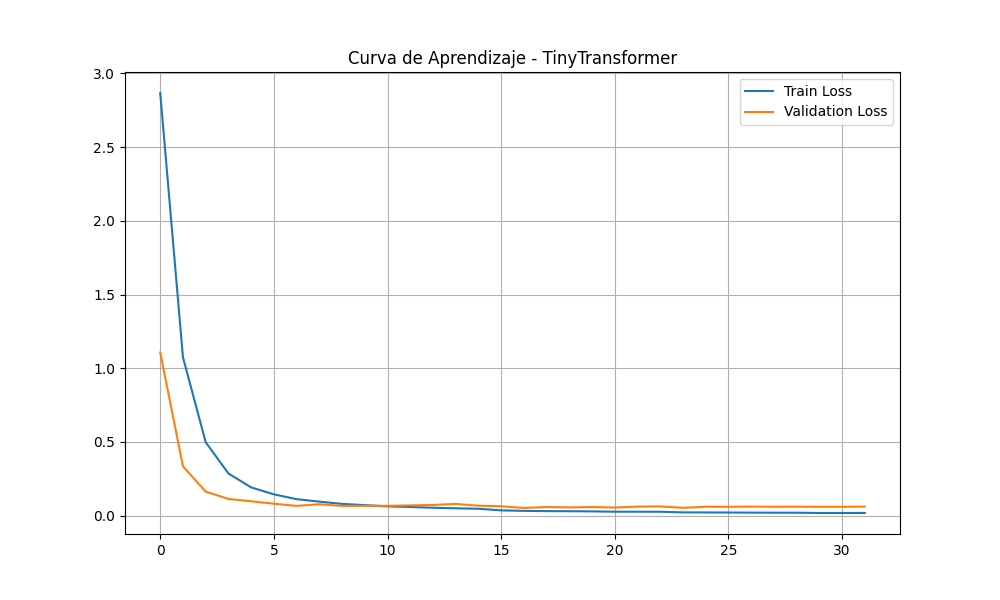
\includegraphics[width=0.82\textwidth]{clasificador/curva_tinyskeleton_final.png}
    \caption{Curva de aprendizaje del reentrenamiento del 21/09/2026 (16 fotogramas, 97 clases). La pérdida de validación mínima fue de $0{,}052$ (exactitud Top-1 fuera de línea del 99{,}14\,\%).}
    \label{fig:curva_final}
\end{figure}

\begin{figure}[H]
    \centering
    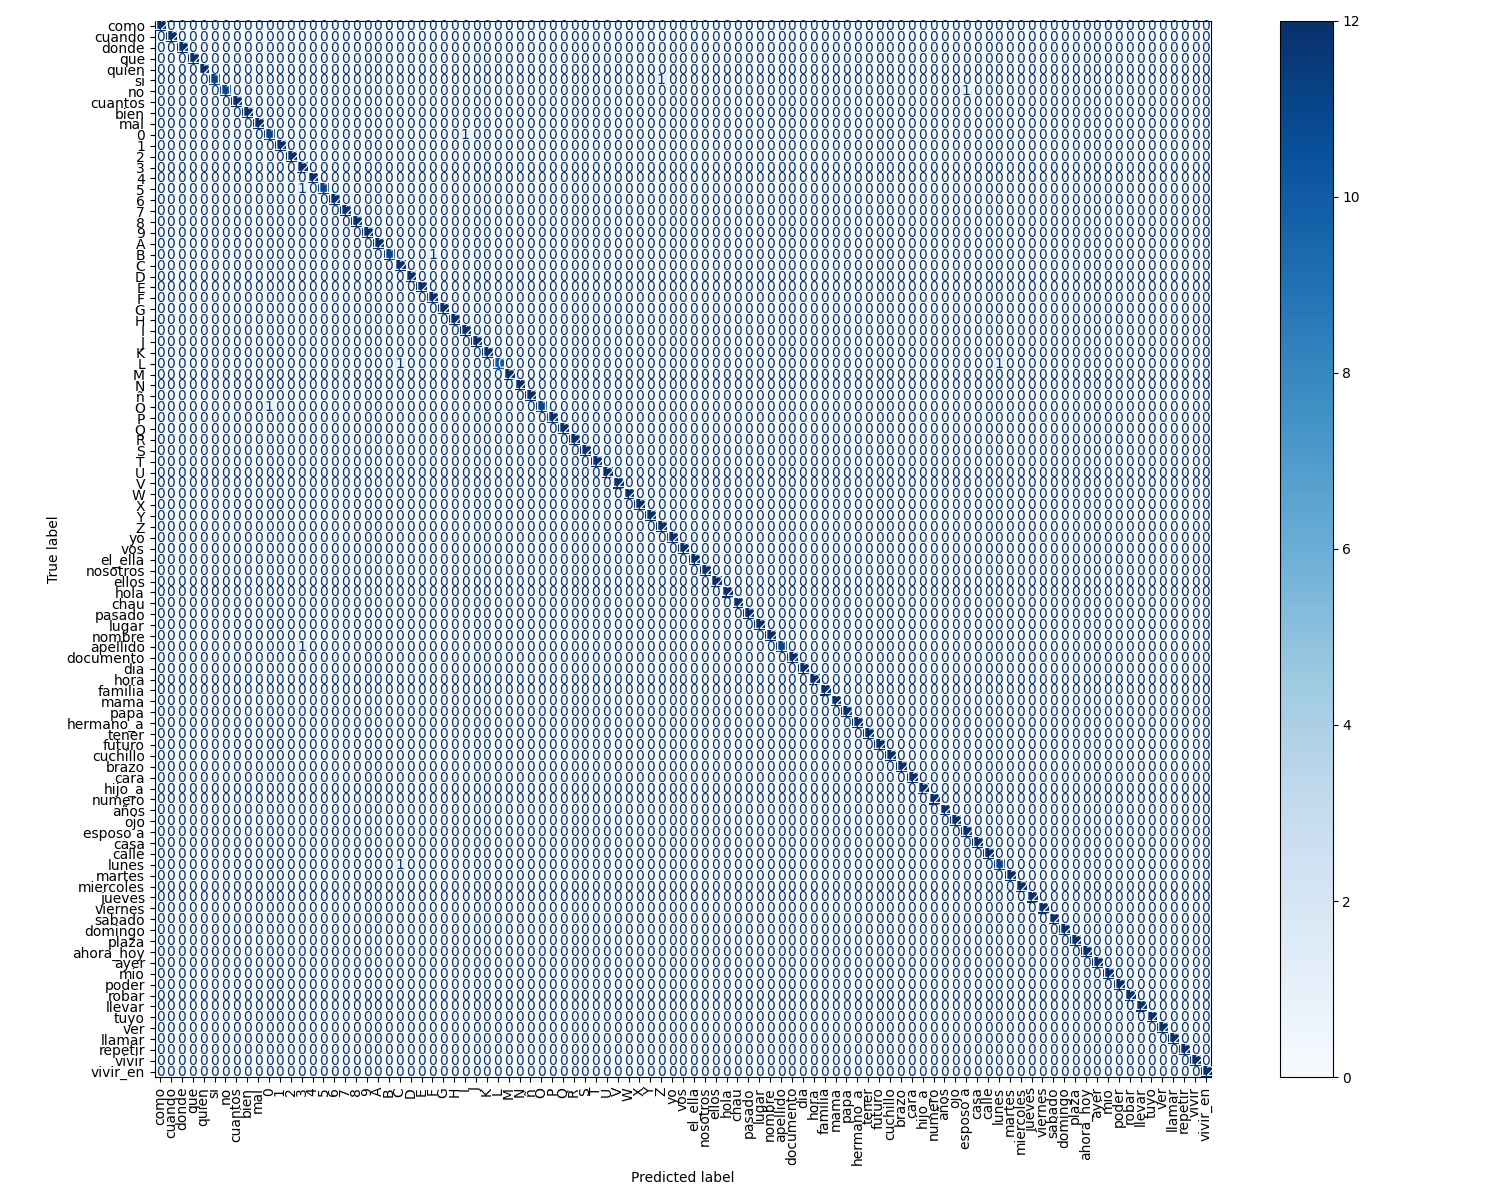
\includegraphics[width=\textwidth]{clasificador/matriz_confusion_final.png}
    \caption{Matriz de confusión en validación fuera de línea para la corrida del 21/09/2026 (97 clases). La concentración de masa en la diagonal refleja la alta separabilidad del dataset estático.}
    \label{fig:matriz_final}
\end{figure}

\begin{figure}[H]
    \centering
    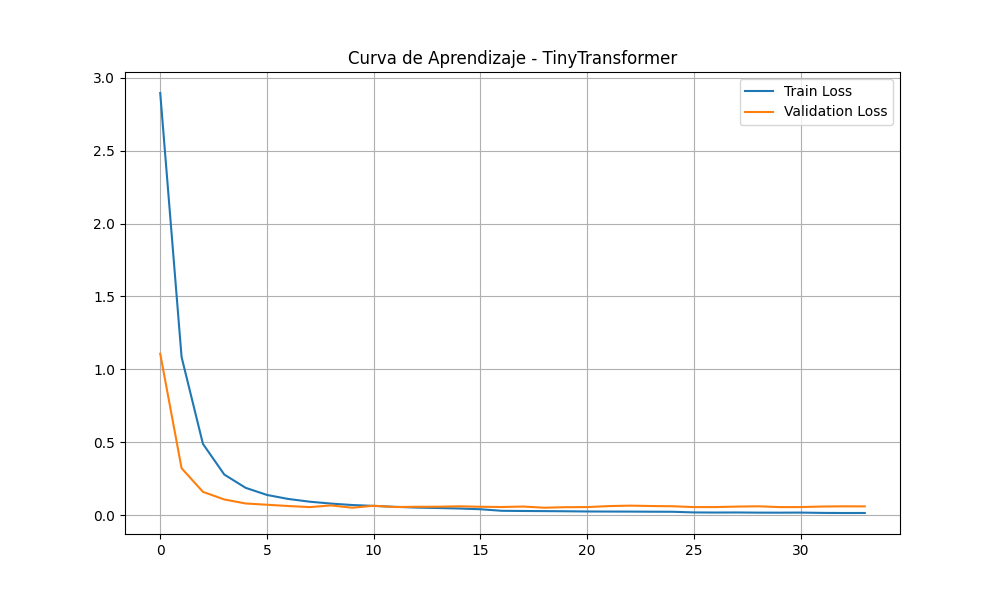
\includegraphics[width=0.82\textwidth]{clasificador/curva_tinyskeleton_100.png}
    \caption{Curva de aprendizaje del reentrenamiento del 15/10/2026 (16 fotogramas, 100 clases), checkpoint integrado en el prototipo. La pérdida de validación mínima, $0{,}0528$, se alcanza en la época 19 (exactitud Top-1 fuera de línea del 99{,}08\,\%).}
    \label{fig:curva_100}
\end{figure}

\section{Evaluación de los módulos de traducción semántica}

Los canales semánticos directo (LSA a español) e inverso (español a LSA) se evaluaron mediante la suite de modelos de lenguaje pequeños (SLM). Cada arquitectura se adaptó mediante LoRA, se fusionó con los pesos base y se cuantizó al formato GGUF preset \texttt{Q4\_K\_M}. La recolección de métricas operó directamente sobre los binarios cuantizados ejecutados en la estación de entrenamiento con aceleración por GPU, con decodificación determinista (temperatura $0$, penalización de repetición $1{,}05$, tope de 24 tokens nuevos en el canal directo).

\subsection{Benchmark comparativo de modelos de lenguaje}
La evaluación de la traducción semántica se estructuró en tres fases:

\paragraph{Primera ronda (julio de 2026).}
Se empleó un conjunto preliminar de cerca de 202 pares de oraciones sintéticas sin validación lingüística. En la Tabla~\ref{tab:slm_julio} se detallan los resultados obtenidos sobre la división 80/20 tras 60 pasos de entrenamiento.

\begin{table}[H]
    \centering
    \small
    \caption{Primera comparación de modelos sobre el corpus sintético preliminar (escala 0--100).}
    \label{tab:slm_julio}
    \begin{tabular}{lccc}
        \toprule
        \textbf{Modelo} & \textbf{BLEU} & \textbf{METEOR} & \textbf{ROUGE-L} \\
        \midrule
        Qwen2.5 0,5B & 9{,}98 & 37{,}08 & 38{,}99 \\
        Qwen2.5 1,5B & 19{,}79 & 49{,}24 & 52{,}09 \\
        Qwen2.5 3B & 48{,}04 & 70{,}87 & 73{,}66 \\
        Llama 3.2 1B & 19{,}62 & 45{,}46 & 47{,}71 \\
        SmolLM2 1,7B & 12{,}46 & 36{,}52 & 35{,}63 \\
        Phi-3-mini-4k & 29{,}21 & 54{,}13 & 57{,}96 \\
        DeepSeek-R1-Distill-Qwen 1,5B & 0{,}00 & 14{,}34 & 6{,}64 \\
        \bottomrule
    \end{tabular}
\end{table}

En esta fase preliminar, Qwen2.5 3B destacó sobre las demás variantes. El modelo DeepSeek-R1-Distill se descartó porque antepone un bloque de razonamiento explícito al texto traducido, y ese bloque anuló el indicador BLEU.

\paragraph{Primera integración en sistema (agosto de 2026).}
El 6 de agosto de 2026 se evaluó el modelo Qwen2.5 3B integrado con el adaptador LoRA mediante la biblioteca PEFT. Sobre un conjunto de prueba de 20 oraciones, alcanzó únicamente 2 aciertos exactos (10\,\%), con un F1 por token de $0{,}50$ y BLEU-4 de $0{,}20$. La inspección cualitativa mostró que el sistema producía paráfrasis válidas que no coincidían literalmente con la única referencia registrada (como «Me siento bien» frente a «Estoy bien»). Esto impulsó la reestructuración del protocolo de evaluación para incorporar múltiples referencias por enunciado.

\paragraph{Rondas de septiembre y octubre de 2026.}
A partir de septiembre se estandarizó el entrenamiento durante 5 épocas ($r=16$, $\alpha=32$, tasa de aprendizaje $5 \times 10^{-4}$, y $3 \times 10^{-4}$ para el modelo de 3B). En la Tabla~\ref{tab:slm_evolucion} se expone la evolución de la exactitud normalizada sobre el 15\,\% reservado a través de las distintas versiones del corpus.

\begin{table}[H]
    \centering
    \small
    \caption{Exactitud normalizada del canal directo sobre el 15\,\% reservado a través de las versiones del corpus.}
    \label{tab:slm_evolucion}
    \begin{tabular}{lcccc}
        \toprule
        \textbf{Modelo} & \textbf{16/09 ($n=99$)} & \textbf{05/10 ($n=123$)} & \textbf{07/10 ($n=115$)} & \textbf{13/10 ($n=119$)} \\
        \midrule
        Qwen2.5 0,5B & 90{,}91\,\% & 91{,}87\,\% & 93{,}04\,\% & 90{,}76\,\% \\
        Qwen2.5 1,5B & 93{,}94\,\% & 96{,}75\,\% & 93{,}04\,\% & 95{,}80\,\% \\
        Qwen2.5 3B & 95{,}96\,\% & 96{,}75\,\% & 89{,}57\,\% & 95{,}80\,\% \\
        Llama 3.2 1B & 93{,}94\,\% & 92{,}68\,\% & 89{,}57\,\% & 93{,}28\,\% \\
        SmolLM2 1,7B & 85{,}86\,\% & 86{,}18\,\% & 90{,}43\,\% & 86{,}55\,\% \\
        \bottomrule
    \end{tabular}
\end{table}

En la corrida del 7 de octubre, Qwen2.5 3B experimentó un fallo de convergencia en la optimización (pérdida residual de $1{,}087$ frente a los valores estándar de $0{,}23$). En todas las evaluaciones válidas, la exactitud estricta coincidió plenamente con la normalizada. Los errores, por lo tanto, correspondieron a variaciones en la selección léxica y no a mayúsculas ni a puntuación.

\subsection{Resultados cuantitativos consolidados}
\label{sec:eval_semantica_cuant}
La evaluación del 13 de octubre de 2026 proporcionó los modelos utilizados en la versión de producción. Las Tablas~\ref{tab:slm_test_1310} y \ref{tab:slm_trial_1310} presentan las métricas sobre el 15\,\% reservado ($n=119$) y sobre el conjunto de prueba fijo (\textit{Trial} de 21 casos con referencias múltiples).

\begin{table}[H]
    \centering
    \small
    \caption{Canal directo: métricas sobre el 15\,\% reservado ($n=119$) para la corrida del 13/10/2026.}
    \label{tab:slm_test_1310}
    \begin{tabular}{lccccc}
        \toprule
        \textbf{Modelo} & \textbf{Exactitud} & \textbf{BLEU} & \textbf{ROUGE-L} & \textbf{METEOR} & \textbf{Latencia} \\
        \midrule
        Qwen2.5 0,5B & 90{,}76\,\% & 95{,}27 & 95{,}34 & 95{,}23 & 125\,ms \\
        Qwen2.5 1,5B & 95{,}80\,\% & 97{,}23 & 97{,}48 & 97{,}11 & 234\,ms \\
        Qwen2.5 3B & 95{,}80\,\% & 98{,}34 & 97{,}59 & 97{,}10 & 429\,ms \\
        Llama 3.2 1B & 93{,}28\,\% & 96{,}47 & 97{,}88 & 97{,}55 & 210\,ms \\
        SmolLM2 1,7B & 86{,}55\,\% & 88{,}29 & 94{,}68 & 94{,}63 & 416\,ms \\
        \bottomrule
    \end{tabular}
\end{table}

\begin{table}[H]
    \centering
    \small
    \caption{Canal directo: métricas sobre el conjunto de prueba fijo (\textit{Trial} de 21 casos con referencias múltiples).}
    \label{tab:slm_trial_1310}
    \begin{tabular}{lcccc}
        \toprule
        \textbf{Modelo} & \textbf{Exactitud} & \textbf{BLEU} & \textbf{METEOR} & \textbf{Latencia} \\
        \midrule
        Llama 3.2 1B & 100{,}00\,\% & 100{,}00 & 99{,}74 & 343\,ms \\
        Qwen2.5 3B & 100{,}00\,\% & 100{,}00 & 99{,}71 & 791\,ms \\
        Qwen2.5 1,5B & 100{,}00\,\% & 100{,}00 & 99{,}69 & 413\,ms \\
        Qwen2.5 0,5B & 100{,}00\,\% & 100{,}00 & 99{,}67 & 226\,ms \\
        SmolLM2 1,7B & 95{,}24\,\% & 97{,}73 & 98{,}74 & 655\,ms \\
        \bottomrule
    \end{tabular}
\end{table}

En el conjunto de reserva, Qwen2.5 1,5B y Qwen2.5 3B empataron en exactitud (95{,}80\,\%) y superaron a Llama 3.2 1B (93{,}28\,\%) y a SmolLM2 (86{,}55\,\%). En la prueba de casos fijos, cuatro modelos alcanzaron el 100\,\% de exactitud y copiaron sin alteraciones los nombres propios, las calles y los números de documento.

\subsection{Análisis de asimetría direccional en el aprendizaje}
Las tareas asociadas a los dos canales de traducción presentan un comportamiento asimétrico:
\begin{itemize}
    \item \textbf{Canal directo (LSA $\rightarrow$ Español):} Corresponde a una tarea de expansión sintáctica. A partir de secuencias de glosas sin conectores ni flexiones, el modelo reconstruye oraciones completas en español.
    \item \textbf{Canal inverso (Español $\rightarrow$ LSA):} Actúa como una tarea de compresión estructurada. A partir de oraciones en español, el modelo mapea los elementos hacia una secuencia rígida de glosas bajo el orden canónico \textit{Topic-Comment}.
\end{itemize}

El despliegue mostró esa especialización de forma directa. Cada canal usa un binario propio. Cuando el binario del canal directo se colocó en lugar del inverso, el servicio respondió a \texttt{/hearing} con una oración en español y no con glosas: el adaptador había aprendido la dirección de la tarea. Las métricas de las corridas del canal inverso no quedaron archivadas, de modo que la comparación entre canales se limita a la naturaleza de cada tarea.

\subsection{Compromiso entre calidad lingüística y latencia de inferencia}
En las pruebas en GPU, la latencia creció con el tamaño del modelo: 125\,ms para Qwen2.5 0,5B, 210\,ms para Llama 3.2 1B, 234\,ms para Qwen2.5 1,5B, 416\,ms para SmolLM2 1,7B y 429\,ms para Qwen2.5 3B. Dado que Qwen2.5 3B no superó la exactitud de Qwen2.5 1,5B y duplicó el tiempo de procesamiento, la arquitectura final seleccionó:
\begin{itemize}
    \item \textbf{Modelo principal:} Qwen2.5 1,5B en formato GGUF \texttt{Q4\_K\_M}, por representar el punto óptimo entre precisión (95{,}80\,\%) y velocidad.
    \item \textbf{Modelo de respaldo (\textit{Fallback}):} Llama 3.2 1B, por su menor huella de memoria y velocidad de inferencia (210\,ms).
\end{itemize}

El despliegue en Google Cloud Run (4 vCPU, 8\,GiB de memoria) aplicó el almacenamiento en caché del prefijo del prompt de contexto ($KV$ cache). La reevaluación completa del prompt en CPU (ante la pérdida de coincidencia del prefijo) demandó cerca de 8 segundos.

\section{Evaluación del sistema integrado y rendimiento en tiempo real}

\subsection{Validación funcional de extremo a extremo}
La integración del prototipo avanzó en cinco hitos funcionales. Desde el segundo, cada uno se verificó de punta a punta en una videollamada de Google Meet:
\begin{enumerate}
    \item \textbf{31 de julio de 2026 (aplicación de escritorio):} La captura y la clasificación de 91 señas corrían en una aplicación con OpenCV, fuera de la videollamada.
    \item \textbf{13 de septiembre de 2026 (extensión web y motor local):} La extensión Manifest V3 y el motor ILSA cerraron el circuito en Google Meet. El traductor Llama 3.2 1B corría en la CPU del equipo, y la oración se mostraba como subtítulo.
    \item \textbf{23 de septiembre de 2026 (servicio semántico remoto):} El motor clasificaba 97 señas, y la traducción pasó a un servidor semántico expuesto mediante un túnel cifrado (\textit{ngrok}).
    \item \textbf{14 y 15 de octubre de 2026 (traductor en la nube y vocabulario de 100 señas):} El servicio semántico pasó a Google Cloud Run, y el motor ILSA incorporó el clasificador de 100 clases con extracción de Holistic en navegador.
    \item \textbf{18 de octubre de 2026 (canal oyente completo):} Se sumó el servicio de poses en Cloud Run. El canal oyente quedó con transcripción local mediante Vosk, estructuración remota en glosas y reproducción del avatar en la videollamada.
\end{enumerate}

Para evaluar la lógica de control del motor local (\texttt{RepeatGate}) y el temporizador de cierre de enunciado, se ejecutó una batería de pruebas resumida en la Tabla~\ref{tab:bateria_logica}.

\begin{table}[H]
    \centering
    \small
    \caption{Resultados de la batería de pruebas sobre la lógica de control del motor local.}
    \label{tab:bateria_logica}
    \begin{tabular}{lll}
        \toprule
        \textbf{Caso de prueba} & \textbf{Entrada ingresada} & \textbf{Resultado emitido} \\
        \midrule
        Dígitos repetidos & \texttt{1 1 1 2 2} & Aceptación total: \texttt{1 1 1 2 2} \\
        Letra repetida tres veces & \texttt{A A A B} & Filtrado a máximo de dos: \texttt{A A B} \\
        Rebote del clasificador & \texttt{HOLA HOLA} & Descarte de duplicado inmediato: \texttt{HOLA} \\
        Repetición no consecutiva & \texttt{HOLA VER HOLA} & Conservación de la secuencia completa \\
        Glosa repetida descartada a los 3\,s & Glosa repetida & El cierre se desplaza a los 7\,s \\
        Movimiento continuo hasta 5\,s & Sin glosa nueva & Cierre de enunciado a los 9\,s \\
        Deletreo dactilológico & \texttt{J U A N} & Conversión directa a «Juan.» sin consulta a nube \\
        Deletreo con ambigüedad & \texttt{T I N A} & Derivación al traductor por coincidencia con \texttt{OJO} \\
        \bottomrule
    \end{tabular}
\end{table}

Durante la integración con la interfaz de Google Meet se corrigieron fallas técnicas de manipulación del flujo multimedia. La Tabla~\ref{tab:fallas_integracion} detalla las anomalías detectadas y la intervención realizada.

\begin{table}[H]
    \centering
    \small
    \caption{Fallas detectadas en la integración con Google Meet y correcciones aplicadas.}
    \label{tab:fallas_integracion}
    \begin{tabularx}{\textwidth}{@{}>{\raggedright\arraybackslash}p{0.42\textwidth} >{\raggedright\arraybackslash}X@{}}
        \toprule
        \textbf{Falla detectada} & \textbf{Intervención de ingeniería aplicada} \\
        \midrule
        Bloqueo del inicio de video en Meet por intercepción permanente de cámara. & Activación del reemplazo de la pista únicamente con el motor ILSA encendido. \\
        \addlinespace[2pt]
        Pérdida de enlace al recargar la extensión con la pestaña de la reunión abierta. & Después de recargar la extensión, se recarga manualmente la pestaña de Meet. \\
        \addlinespace[2pt]
        Detección de falsas manos provocada por movimiento del torso. & Exigencia de un número mínimo de cuadros consecutivos con mano detectada antes de abrir el gesto. \\
        \addlinespace[2pt]
        Interferencia en la captura por movimiento de personas en el fondo. & Delimitación del área de actividad basada exclusivamente en los puntos articulares de las manos. \\
        \addlinespace[2pt]
        Latencia por baja tasa de cuadros en umbrales estáticos. & Conversión de las reglas de espera de recuento de fotogramas a milisegundos reales. \\
        \addlinespace[2pt]
        Sobrecarga de CPU en la transferencia de imágenes hacia la ventana \textit{offscreen}. & Reducción de la resolución de los cuadros transferidos a $240$ píxeles de ancho con compresión ajustada. \\
        \addlinespace[2pt]
        El ejecutable no abría en equipos sin el entorno de Visual C++ ni encontraba las bibliotecas de PyTorch. & Inclusión de las bibliotecas dinámicas requeridas dentro de la carpeta de distribución del ejecutable. \\
        \bottomrule
    \end{tabularx}
\end{table}

\subsection{Análisis de latencias totales por etapa del pipeline}
\label{sec:latencias_pipeline}
El tiempo de respuesta percibido en el canal directo integra retardos de procesamiento numérico y pausas configuradas en la lógica del sistema. La Tabla~\ref{tab:latencias_etapas} detalla la contribución de cada etapa.

\begin{table}[H]
    \centering
    \small
    \caption{Desglose de los componentes del retardo en el canal directo.}
    \label{tab:latencias_etapas}
    \begin{tabularx}{\textwidth}{@{}>{\raggedright\arraybackslash}p{0.32\textwidth} >{\raggedright\arraybackslash}p{0.20\textwidth} >{\raggedright\arraybackslash}X@{}}
        \toprule
        \textbf{Etapa del pipeline} & \textbf{Duración / Retardo} & \textbf{Naturaleza del parámetro} \\
        \midrule
        Detección de fin de seña & $\approx 0{,}4$\,s & Configurado (12 fotogramas sin manos). \\
        Inferencia del clasificador & $0{,}78$\,ms (CPU) / $1{,}08$\,ms (GPU) & Medido el 31/07 sobre el modelo de 32 fotogramas y 91 clases. \\
        Separación mínima entre señas & $1{,}0$\,s & Configurado (tiempo de reposo inter-gestual). \\
        Pausa de cierre de enunciado & $4{,}0$\,s & Configurado (inactividad para disparar traducción). \\
        Generación de oración (LLM) & $234$\,ms & Medido fuera de línea en GPU para Qwen2.5 1,5B; no representa el servicio en Cloud Run. \\
        Reevaluación de prompt (CPU) & $\approx 8$\,s & Valor típico observado en CPU ante pérdida de caché $KV$. \\
        Arranque en frío del servicio & $1$--$3$\,min & Ocurre únicamente si la instancia escaló a cero. \\
        Permanencia de subtítulo & $8{,}0$\,s & Configurado (visibilidad en lienzo virtual). \\
        \bottomrule
    \end{tabularx}
\end{table}

El componente determinante de la espera en la comunicación es la pausa fija de 4,0 segundos, introducida deliberadamente para asegurar la conclusión del enunciado en LSA antes de consultar al modelo de lenguaje.

\subsection{Consumo de recursos de hardware: máquina de desarrollo frente a equipo objetivo}
\label{sec:hardware_objetivo}
En la Tabla~\ref{tab:hw_comparacion} se detalla el comportamiento del sistema evaluado sobre las dos plataformas de hardware del proyecto durante la versión con traductor local (13 de septiembre de 2026).

\begin{table}[H]
    \centering
    \small
    \caption{Comparativa de desempeño del sistema según la plataforma de hardware (con traductor local).}
    \label{tab:hw_comparacion}
    \begin{tabularx}{\textwidth}{@{}>{\raggedright\arraybackslash}p{0.25\textwidth} >{\raggedright\arraybackslash}X >{\raggedright\arraybackslash}X@{}}
        \toprule
        \textbf{Componente} & \textbf{Estación de desarrollo (GPU)} & \textbf{Equipo objetivo (Laptop sin GPU)} \\
        \midrule
        Extracción MediaPipe & Fluida dentro de Meet. & Pocos fotogramas por segundo; umbrales de captura reajustados en milisegundos. \\
        Clasificador local & Menos de 2\,ms por inferencia (medido). & Sin demora perceptible (observación cualitativa). \\
        Traductor local & Respuesta fluida. & Espera perceptible, incompatible con el ritmo de una llamada. \\
        \bottomrule
    \end{tabularx}
\end{table}

Esta evaluación motivó la reestructuración de la arquitectura: el clasificador permaneció en el cliente de borde (cerca de $1{,}66$\,MB para sus 414\,309 parámetros), mientras que el modelo de lenguaje se reubicó en un servicio remoto en Google Cloud Run.

\section{Discusión técnica y lecciones de ingeniería aprendidas}

El desarrollo y la evaluación experimental del prototipo permitieron extraer las siguientes lecciones de ingeniería de software y aprendizaje profundo:

\begin{enumerate}
    \item \textbf{La evaluación fuera de línea no garantiza el rendimiento en entorno real:} Aunque la validación estática superó el 96\,\% de exactitud en todas las iteraciones, la precisión del clasificador disminuyó al enfrentarse a la variabilidad de la cámara web. Las decisiones de selección debieron guiarse por las pruebas en vivo.
    \item \textbf{La evaluación semántica exige referencias múltiples:} La utilización de una única referencia de traducción penalizó paráfrasis válidas en español. La incorporación de referencias múltiples corrigió este artefacto de medición.
    \item \textbf{La calidad del dataset fue el factor determinante:} Las mejoras principales en la traducción semántica no provinieron de un modelo de lenguaje más grande. Provinieron de la depuración del corpus, de la reestructuración del etiquetado y de la introducción de tokens unificados para nombres propios y números.
    \item \textbf{Prevención de errores silenciosos de configuración:} La compatibilidad de formas matriciales en entornos como PyTorch puede ocultar discrepancias en la cantidad de cabezas de atención entre la instanciación y el entrenamiento. Esa discrepancia altera las probabilidades sin emitir excepciones. Por este motivo, la configuración debe serializarse y validarse junto con el checkpoint.
    \item \textbf{Gestión de la memoria conversacional:} La inclusión de turnos previos en el prompt distanció las entradas de la distribución de entrenamiento aprendida por los adaptadores LoRA. La traducción por enunciados independientes garantizó la estabilidad de las respuestas.
    \item \textbf{Impacto de la arquitectura híbrida:} La delegación de la traducción semántica a la nube resolvió la carga de cómputo del traductor en el equipo cliente. A cambio, introdujo la dependencia de la latencia de red y el tiempo de arranque en frío del servicio.
    \item \textbf{Trabajos y mediciones pendientes:} Se identificó la necesidad de completar mediciones futuras que incluyan la caracterización de latencias de extremo a extremo con percentiles a partir de los registros del motor local, la recolección de métricas de uso de CPU/RAM en cliente con la traducción remota, la compilación de resultados del canal inverso y la ejecución de pruebas de usabilidad con usuarios sordos.
\end{enumerate}